\documentclass[accentcolor=tud9c,colorbacktitle,inverttitle,landscape,german,presentation,t]{tudbeamer}
\usepackage{amstext}
\usepackage{amsmath}
\usepackage{graphicx}
\usepackage{multicol}
\usepackage{mathtools}
\usepackage{subfigure}
\usepackage[ngerman,english]{babel}
\usepackage[utf8]{inputenc}
\usepackage{colortbl}
\usepackage{adjustbox}

\begin{document}

\title{\"Ubung 9 - Gruppe 142}
\subtitle{Visual Computing - 3D-Visualisierung}

\author[Johannes Beck, Christian Eilers, Robin Menzenbach, Martin Steinborn]{Johannes Beck, Christian Eilers, Robin Menzenbach, Martin Steinborn}


\date{\today}

\begin{titleframe}
\end{titleframe}

\section{Aufgabe 1}
	\begin{frame}
		\frametitle{Aufgabe 1: 3D-Daten}
		3D-Daten können nicht nur Gewonnen, sondern auch genutzt werden, um Dinge dar- oder herzustellen. Beispiele hierfür wären 3D Drucker oder CAD Software.
		
	\end{frame}

\section{Aufgabe 2}
\begin{frame}
	\frametitle{Aufgabe 2: Volumenvisualisierung}
			\begin{itemize}
			\item[a)]
			Abbildung 1: Direkte Volumenvisualisierung \\
			Abbildung 2: Indirekte Volumenvisualisierung \\
			\textbf{Direkte Volumenvisualisierung:} Die Visualisierung des 3D-Objekts funktioniert ohne die Generierung einer Metadarstellung. Hierfür wird die Emission und Absoption bei durchschicken eines Strahls durch das Objekt betrachtet. \\
			\textbf{Indirekte Volumenvisualisierung:} Es wird zunächst eine Zwischendarstellung des Volumens generiert. Hierfür können zB. mithilfe des Marching-Cubes Algorithmus Isoflächen erzeugt werden, aus welchen später die Visualisierung des Objekts erfolgt.
			\item[b)]
			Bei sehr großen Oberflächen bietet es sich an unsichtbare Polygone zu entfernen und die Gesamtanzahl der Polygone zu verringern. Die hierfür verwendeten Methoden sind das Culling und die Meshreduktion.
	\end{itemize}
\end{frame}
\begin{frame}
	\frametitle{Aufgabe 2: Volumenvisualisierung}
	\begin{itemize}
		\item[c)]
			\begin{itemize}
			\item Backface-Culling: Polygone, bei denen lediglich die Rückseiten sichtbar sind (Polygonnormale zeigen vom Sichtpunkt werg), werden nicht gezeichnet. \\
			\item View-Frustum-Culling: PÜolygone, welche zum teil oder vollständig außerhalb des View-Frustums liegen werden nur zum Teil oder überhaupt nicht gezeichnet.\\
			\item Occlusion-Culling:Polygone werden nach Tiefe sortiert und nur gerendert wenn sie unter beachtung der Transparenz der überliegenden Polygone nicht vollständig verdeckt sind.\\
			\end{itemize}
		
		\item[d)] Es wird ein Mesh berechnet, der die Oberfläche repräsentiert.
	\end{itemize}
\end{frame}

\section{Aufgabe 3}
\begin{frame}
	\frametitle{Aufgabe 3: Voronoi-Diagramme}
	\begin{itemize}
	\item[a)]
	Die Delauney-Triangulierung des angegebenen Diagramms ist in Abbildung \ref{DelTri} abgebildet. Wie man sehen kann enthält der Umkreis eines jeden Dreiecks lediglich die eigenen Punkte und keine Weiteren. Somit liegt eine korrekte Delauney-Triangulierung vor.
	\begin{figure}
		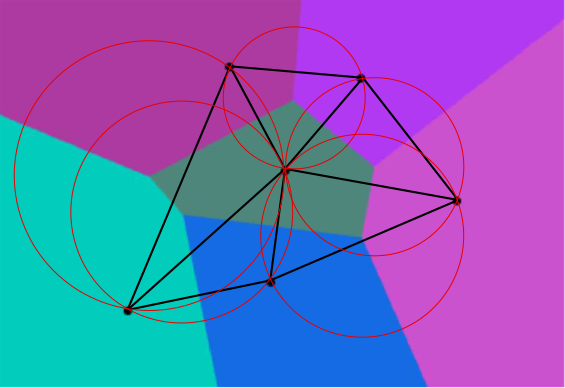
\includegraphics[width = .5\linewidth]{task_3a.png}
		\caption{Delauney-Triangulierung des gegebenen Diagramms}
		\label{DelTri}
	\end{figure}
	\end{itemize} 
\end{frame}
\begin{frame}
	\frametitle{Aufgabe 3: Voronoi-Diagramme}
	\begin{itemize}
	\item[b)]
	Bei der Erstellung einer Delauney-Triangulierung muss Edge-Flipping angewendet werden, wenn der Umkreis eines Dreiecks einen Punkt eines anderen Dreiecks einschließt. Da dies nicht zulässig ist, wird die gemeinsame Kante der beiden Dreiecke gelöst und die beiden anderen Punkte verbunden. Diesen Vorgang nennt man Edge-Flipping. Ist lediglich eine Punktmenge als ausgangspunkt gegeben, kann diese zu beliebigen Dreiecken(ohne Kantenüberschneidung)  verbunden werden, welche dann mittels Edge-Flipping an Fehlerhaften Stellen in eine Delauney-Triangulierung überführt werden kann. 
	\end{itemize} 
\end{frame}

\section{Aufgabe 4}
\begin{frame}
	\frametitle{Aufgabe 4: Volume Rendering und Marching Cubes}
	\begin{itemize}
	\item[a)]
		\begin{itemize}
			\item Marching-Cubes: Die Anzahl zu berechnender Polygone \\
			\item Ray-Casting: Anzahl der Voxel und der Auflösung der Anzeigefläche
		\end{itemize}
	\item[b)] %TODO: Nennen Sie einen Vor- und einen Nachteil von Volume Rendering gegenüber Marching Cubes.
	\begin{itemize}
		\item Vorteil: Das Rendern der kompletten Daten erhält Informationen, welche beim Rendern der lediglich sichtbaren Oberfläche verloren gehen. \\
		\item Nachteil: Da beim Volume Rendering nicht nur die Sichtbare Oberfläche gerendert wird wie beim Marching Cubes Algorithmus entsteht ein höherer Berechnungsaufwand.
	\end{itemize}
	\end{itemize}
\end{frame}

\section{Aufgabe 5}
\begin{frame}
	\frametitle{Aufgabe 5: Marching Squares}
	\begin{itemize}
		\item[a)] Es wird die Isolinie für den gegebenen Isowert berechnet, sie verbindet Datenpunkte mit gleichen Werten.
		\item[b)]
		Die Abbildung zeigt die Anwendung des Marching Squares Algorithmus mit Isowert 31 auf das vorgegebene Feld. Die Werte innerhalb des Isofläche wurden grau hinterlegt, sowie deren Umrandung in schwarz eingefügt.
		\begin{figure}
			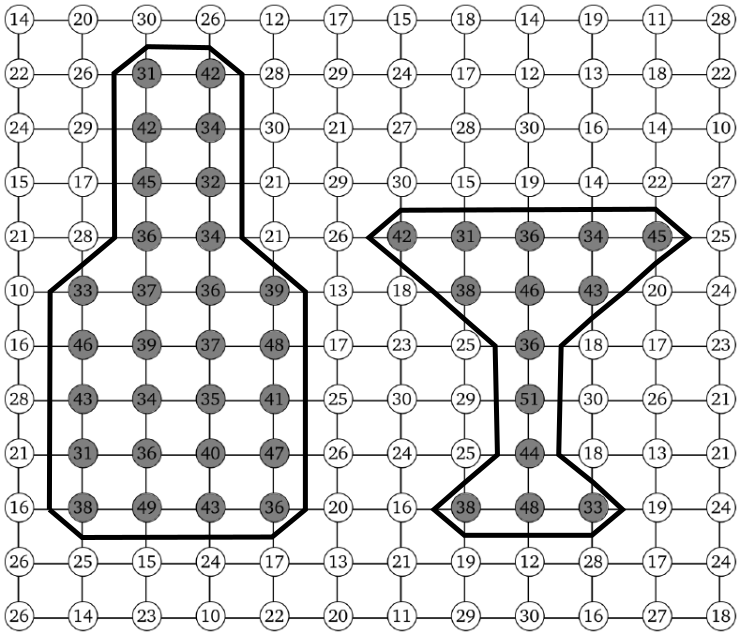
\includegraphics[width = .4\linewidth]{task_5b.png}
			\label{MaSq}
		\end{figure}
	\end{itemize}
\end{frame}
\end{document}
